\documentclass[a4paper,12pt]{jreport}
\usepackage[dvipdfmx]{graphicx}
\usepackage{mymacros}
\usepackage{here}
\usepackage{morefloats}
\textheight 9.0in
\textwidth 6.0in
\topmargin 0in
\oddsidemargin .2in
\evensidemargin .2in
\title{
{\LARGE\sffamily\gtfamily
修\ \ 士\ \ 論\ \ 文\\
}
\vspace*{.6in}
{\huge\sffamily\gtfamily
OJLによるトレースログ可視化ツールの開発\\
}
\vfill\vfill\vfill
}
\author{
\LARGE\sffamily\gtfamily
350702101\ \ \ \ 後藤 隼弐\\
}
\date{
\vfill
\Large\sffamily\gtfamily
名古屋大学 大学院情報科学研究科\\[.2in]
情報システム学専攻\\[.2in]
2009年1月
\vfill
}
\renewcommand{\bibname}{参考文献}
\renewcommand{\baselinestretch}{1.075}
\begin{document}
\pagestyle{empty}
%%%%%%%%%%%%%%%%%%%%%%%%%%%%%%%%%%%%%%%%%%%%%%%%%%%%%%%%%%%%%%%%%%%%%%%%%%
% 和文要旨
%-------------------------------------------------------------------------
\vspace*{-1in}
\begin{center}
\Large\sffamily\gtfamily OJLによるトレースログ可視化ツールの開発
\end{center}
\begin{flushright}
\large\sffamily\gtfamily
350702101\ \ \ \ 後藤 隼弐
\end{flushright}
\begin{center}
\large\sffamily\gtfamily 要旨
\end{center}
{
\setlength{\baselineskip}{0.9\normalbaselineskip}

要旨

}
\clearpage
%%%%%%%%%%%%%%%%%%%%%%%%%%%%%%%%%%%%%%%%%%%%%%%%%%%%%%%%%%%%%%%%%%%%%%%%%%
% 英文要旨
%-------------------------------------------------------------------------
\vspace*{-1in}
\begin{center}
\Large\sffamily
Development of Visualization Tool for Trace Log by OJL
\end{center}
\begin{flushright}
\large\sffamily\gtfamily
350702101\ \ \ \ Junji Goto
\end{flushright}
\begin{center}
\large\sffamily Abstract
\end{center}
{
\setlength{\baselineskip}{0.9\normalbaselineskip}

In recent years, multiprocessors have been used even in embedded systems.
The reason for this is limits of effectiveness that improve a performance through overclocking in a single processor.
A multiprocessor system can reduce the increase in power consumption even though improving performance by parallel processing.
However, there is a problem that it is difficult to debug software executed in multiprocessors.
This means that a traditional debugging way using breakpoints and step excuting is ineffective, because a repeatability of bug is made low by a nondeterministic behavior of parallel processing.

On the other hand, an effective technique to debug software excuted in multiprocessors includes analyzing a trace log that is a program execution history.
The reason for that the technique is effective is that it can know necessary information for a parallel program debugging by analyzing the trace log.
The information, for example, are when, where or how long processes executed.
However, it is inefficient that developeres analyze the trace log directly, because searching a desired information in tremendous quantities of trace log and analyzing time-series trace log recorded by a number of processors sequentially are difficult.

Techniques to support developeres to analyze the trace log includes visualizing trace log by tools.
And, many visualizing tools for trace log have been developed before now.
In particular, there are debugging software or integrated development environment for embedded systems and trace log profilers for Unix-like operating systems.
However, these existing tools lack general versatility because they treat only own format trace log. 
And, they lack expandability because visualized information are limited to items provided by them.

To that end, we developed TraceLogVisualizer(TLV), a visualization tool forthe trace log, for the purpose of implementation of general versatility and expandability.
First, we defined the standard-format-trace-log with generalizing a trace log.
This is necessity for that the TLV treat the trace log abstractively.
And, we provided a mechanism that any format trace logs convert to the standard-format-trace-log by writing a convert-rule-file.
Next, we formalized a mechanism associating shapes and trace logs as visualize-rule-file through abstracting them.

We confirmed general versatility through attemptting to visualize trace logs of a wide variety of formats including the trace log of RTOS (Real-time operating system) for a singlecore processor and multicore processors, and embedded component systems.
Also, we confirmed expandability through attemptting to add and change visualized information.
In the result, they are achieved by writing convert-rule-files and visualize-rule-files.

Development of TLV was performed as OJL(On the Job Learning), and development process carried out by applying use case driven agile development.

}
\clearpage
%%%%%%%%%%%%%%%%%%%%%%%%%%%%%%%%%%%%%%%%%%%%%%%%%%%%%%%%%%%%%%%%%%%%%%%%%%
% 中表紙
%-------------------------------------------------------------------------
\maketitle
\clearpage
%%%%%%%%%%%%%%%%%%%%%%%%%%%%%%%%%%%%%%%%%%%%%%%%%%%%%%%%%%%%%%%%%%%%%%%%%%
% 目次
%-------------------------------------------------------------------------
\pagestyle{plain} \pagenumbering{roman}
\setcounter{page}{1}
\tableofcontents
\listoffigures
\listoftables
\clearpage
%%%%%%%%%%%%%%%%%%%%%%%%%%%%%%%%%%%%%%%%%%%%%%%%%%%%%%%%%%%%%%%%%%%%%%%%%%
% 本文
%-------------------------------------------------------------------------
\pagestyle{plain} \pagenumbering{arabic}
\setcounter{page}{1}
%%%%%%%%%%%%%%%%%%%%%%%%%%%%%%%%%%%%%%%%%%%%%%%%%%%%%%%%%%%%%%%%%%%%%%%%%%
\chapter{はじめに}

\section{開発背景}

近年,PC,サーバ,組み込みシステム等,用途を問わずマルチプロセッサの利用が進んでいる.
その背景には,シングルプロセッサの高クロック化による性能向上効果の停滞や,消費電力・発熱の増大がある.
マルチプロセッサシステムでは処理の並列性を高めることにより性能向上を実現するため,消費電力の増加を抑えることが出来る.
組み込みシステムにおいては,機械制御とGUIなど要件の異なるサブシステム毎にプロセッサを使用する例があるなど,従来から複数のプロセッサを用いるマルチプロセッサシステムが存在していたが,部品点数の増加によるコスト増を招くため避ける方向にあった.
しかしながら,近年は,1つのプロセッサ上に複数の実行コアを搭載したマルチコアプロセッサの登場により低コストで利用することが可能になり,低消費電力要件の強い組み込みシステムでの利用が増加している.

マルチプロセッサ環境でソフトウェアを開発する際に問題になる点として,デバッグの困難さが挙げられる.
これは,処理の並列性からプログラムの挙動が非決定的になり,バグの再現が保証されないため,シングルプロセッサ環境で用いられているブレークポイントやステップ実行を用いた従来のデバッグ手法が有効でないからである.

一方,マルチプロセッサ環境で有効なデバッグ手法として,プログラム実行履歴であるトレースログを解析する手法が挙げられる.
この手法が有効である理由は,並列プログラムのデバッグにおいて必要な情報である,各プロセスが,いつ,どのプロセッサで,どのくらい動作していたかということを,トレースログを解析することで知ることが出来るからである.
しかしながら,開発者が直接トレースログを解析するのは効率が悪い.
これは,膨大な量となるトレースログから所望の情報を探し出すのが困難であることや,各プロセッサのログが時系列に分散して記録されるため,逐次的にログを解析することが困難であることが理由である.

しかしながら,トレースログを開発者が直接扱うのは困難である場合が多い.
これは,ログの情報の粒度が細かくなるほど単位時間あたりのログの量が増える傾向にあり,膨大なログから所望の情報を探し出すのが困難であることや,各コアのログが時系列に分散して記録されるため,逐次的にログを解析することが困難であるからである.
そのため,トレースログの解析を支援するツールが要求されており,ログを解析し統計情報として出力したり,可視化表示することで開発者の負担を下げる試みが行われている.

\section{既存のトレースログ可視化ツール}

既存のトレースログ可視化表示ツールとしては,組込みシステム向けデバッガソフトウェアや統合開発環境の一部,Unix系OSのトレースログプロファイラ,波形表示用ツールの流用などがある.

本節では,これら既存のトレースログ可視化ツールについて説明した後,これらの問題点について指摘する.

\subsection{組み込みシステム向けデバッガソフトウェア}

組み込みシステム向けデバッガソフトウェアには,機能の1つとしてトレースログを可視化する機能が含まれている場合がある.
組み込みシステム向けデバッガソフトウェアとは,ICE(In-Circuit Emulator)やJTAGエミュレータなどの,組み込みシステム向けデバッガに付属するデバッグ用のソフトウェアである.
ここで,組み込みシステム向けデバッガとは,ターゲットシステム上で動くプログラムをホストシステム上でデバッグを行えるようにするために,ターゲットCPUにアクセスする手段を提供する装置を指す.

組み込みシステム向けデバッガソフトウェアとしては,京都マイクロコンピュータ株式会社のPARTNER\cite{PARTNER-JET}や,株式会社ソフィアシステムズのWatchPoint\cite{watchpoint}などがあり,それぞれ,イベントトラッカー,OSアナライザというトレースログを可視化する機能を提供している.
図\ref{fig:PARTNER-JET}に,イベントトラッカーのスクリーンショットを,図\ref{fig:watchpoint}にOSアナライザのスクリーンショットを示す.

これら組み込みシステム向けデバッガソフトウェアの一機能としての可視化ツールは,その性質からターゲットとなるOSやプロセッサが限定される.
これは,組み込みシステム向けデバッガは通常,ターゲットとなるプロセッサが限られており,デバッガソフトウェアが対応するOSも限られているからである.
また,可視化表示したい情報も提供されているものに限られるなど,可視化ツールとしては汎用性,拡張性に乏しい.

\begin{figure}[p]
\begin{center}
\includegraphics[height=9cm]{img/PARTNER-JET.eps}
\caption{PARTNER イベントトラッカー}
\label{fig:PARTNER-JET}
\end{center}
\end{figure}

\begin{figure}[p]
\begin{center}
\includegraphics[height=4cm]{img/watchpoint.eps}
\caption{WatchPoint OSアナライザ}
\label{fig:watchpoint}
\end{center}
\end{figure}

\subsection{組み込みOS向けの統合開発環境}

QNX Software Systems社は,自社の組み込みリアルタイムオペレーティングシステムQNXの統合開発環境としてQNX Momenticsを販売している.QNX Momenticsにはシステムプロファイラとして,システムコールや割込み,スレッド状態やメッセージなどを可視化するQNX System Profiler\cite{QNXMomentics}という機能を提供している.図\ref{fig:QNXSystemProfiler}にQNX System Profilerのスクリーンショットを示す.

また,イーソル株式会社はT-Kenel/$\mu$ITRONベースシステムの統合開発環境としてeBinder\cite{eBinder}を販売している.eBinderにはイベントログ取得・解析ツールとしてEvenTrekが付属しており,システムコール,割込み,タスクスイッチ,タスク状態遷移などを可視化することが出来る.図\ref{fig:EvenTrek}にQNX System Profilerのスクリーンショットを示す.

このように,商用の組み込みOS向けの統合開発環境にはOSの実行履歴を可視化表示する機能が搭載されている場合がある.しかしながらこれらは,各ベンダーが自社OSの競争力を高めるために提供されているものであり,当然ながら可視化表示に対応するOSは自社提供のものに限られている.
また,可視化表示する情報も提供するものに限られており,表示のカスタマイズ機能もそれほど自由度は高くはない.

\begin{figure}[p]
\begin{center}
\includegraphics[height=9cm]{img/QNXSystemProfiler.eps}
\caption{QNXSystemProfiler}
\label{fig:QNXSystemProfiler}
\end{center}
\end{figure}

\begin{figure}[p]
\begin{center}
\includegraphics[height=9cm]{img/EvenTrek.eps}
\caption{eBinder EvenTrek}
\label{fig:EvenTrek}
\end{center}
\end{figure}

\subsection{Unix系OSのトレースログプロファイラ}

Unix系OSでは,これまでに,パフォーマンスチューニングや障害解析を目的として,カーネルの実行トレースを取得するソフトウェアがいくつか開発されている.
ここでは,単にこれをトレースツールと呼称する.

Linux用のトレースツールとしてはLKST\cite{LKST},SystemTap\cite{SystemTap},LTTng\cite{LTTng}などがあり,Solaris用にはDtrace\cite{Dtrace}がある.
これらトレースツールが提供する主な機能は,カーネル内にフックを仕込みカーネル内部状態をユーザー空間に通知する機能,通知をログとして記録する機能である.

これらのトレースツールは,ログを分析,提示する,専用のプロファイラツールを提供している場合が多い.
たとえば,LTTngにはLTTV\cite{LTTV}が,DTraceにはChime\cite{Chime}が,プロファイラツールとして提供されている.
図\ref{fig:LTTV}にLTTVのスクリーンショットを,図\ref{fig:Chime}にChimeのスクリーンショットを示す.

これら,プロファイラツールは,主に,カーネルの内部状態を統計情報として出力することにより,ボトルネックを探したり,障害の要因を探る目的で使用されるが,ソフトウェアのデバッグを目的に使用することもできる.
DTraceなどはログ出力のためのカーネルフックポイントを独自のスクリプト言語を用いて制御できるなど,任意の情報をソフトウェアの実行から取得することができる.
しかしながら,取得したログを任意の図形で可視化する手段は提供されておらず,テキスト形式での確認となる.
また,可視化表示する際のログの形式は,そのOSのトレースツールが出力する形式に依存するため,他のOSのトレースを可視化することはできない.

\begin{figure}[p]
\begin{center}
\includegraphics[height=9cm]{img/LTTV.eps}
\caption{LTTV}
\label{fig:LTTV}
\end{center}
\end{figure}

\begin{figure}[p]
\begin{center}
\includegraphics[height=9cm]{img/Chime.eps}
\caption{Chime}
\label{fig:Chime}
\end{center}
\end{figure}

\subsection{波形表示ツールの流用}

任意のOS,アプリケーションのトレースログを可視化表示する手段として,波形表示ツールを流用する方法がある.
波形表示ツールとは,Verilog等のデジタル回路設計用論理シミュレータの実行ログを波形で表示するソフトウェアのことを指す.

デジタル回路設計用論理シミュレータの実行ログには,VCD(Value Change Dump)形式というオープンなファイルフォーマットが存在する.
そのため,任意のログをVCD形式として出力することにより,これらのツールで可視化表示することが可能になる.
図\ref{fig:GTKWave}に,VCD形式のログの可視化に対応した波形表示ツールGTKWaveのスクリーンショットを示す.

波形表示ツールを流用する方法では,任意のログをオープンフォーマットなファイル形式に変換することによりログの形式に依存せずに利用できる反面,表示能力に乏しく,複雑な可視化表現は難しいという問題がある.

\begin{figure}[p]
\begin{center}
\includegraphics[height=9cm]{img/GTKWave.eps}
\caption{GTKWave}
\label{fig:GTKWave}
\end{center}
\end{figure}

\subsection{既存のトレースログ可視化ツールの問題点}

既存のトレースログ可視化ツールは,可視化ツールとして単体で存在しているわけではなく,トレースログを出力するソフトウェアの一部として提供されている.
そのため,読み込めるトレースログの形式が出力ソフトウェアに依存しており,可視化対象となるOS,プロセッサが制限されてしまっている.

読み込むトレースログの形式を制限しないためには,波形表示ツールのようにトレースログ可視化ツール用に標準化されたトレースログ形式を定める必要があると考えられるが,現状,公表されているものではそのようなものは確認できていない.

ログ形式の標準化としては,syslog\cite{RFC3164}と呼ばれる,ログメッセージをIPネットワーク上で転送するための標準規格がRFC3164として策定されており,その一部にログ形式について規定されている.
しかしながら,syslogにおけるログ形式は,時刻の最小単位が秒であり,デバッグを目的に利用するには粒度が粗く,また,メッセージ内容がフリーフォーマットであるなど,自由度が高すぎるため,可視化ツールが読み込むログの標準形式としては不適切である.

既存のトレースログ可視化ツールのもうひとつの問題点としては,可視化表示の項目や形式が,提供されているものに限られていることが挙げられる.
既存のトレースログ可視化ツールで可視化表示の項目を追加,変更したり,可視化表現をカスタマイズする機能を搭載するものは確認できていない.

\section{開発目的と内容}

前節で説明したとおり,既存のトレースログ可視化ツールには,標準化されたトレースログ形式がないことによりターゲットが限定されてしまっているという,汎用性に乏しい点と,可視化表示項目が提供されているものに限られているという,拡張性に乏しい点の2つの問題点があることを指摘した.

そこで我々は,これらの問題点を解決し,汎用性と拡張性を備えたトレースログ可視化ツールを開発することを目的とし,TraceLogVisualizer (TLV) を開発した.

はじめに,TLVの内部でトレースログを抽象的に扱えるよう,トレースログを一般化した標準形式トレースログを定めた.
次に,任意の形式のトレースログを標準形式トレースログに変換する仕組みを変換ルールとして形式化した.
この変換ルールを外部ファイルとして与えることで,任意の形式のトレースログを読み込めるようになる.

また,トレースログの可視化表現を指示する仕組みを抽象化し,可視化ルールとして形式化した.
この可視化ルールも,同じように外部ファイルとして与えることで,可視化表示項目の追加や変更,可視化の表現方法を自由に設定することが出来るようになる.

TLVでは,このように,変換ルールと可視化ルールを外部ファイルとして与えることで,汎用性と拡張性を実現した.

\section{論文の構成}
本節では本論文の構成を述べる.

2章では,TLVの設計について述べる.
ここでは,問題解決のために開発方針をどのように設定したかを述べ,具体的な解決策をどのように設計したかを述べる.
3章では,TLVの実装について述べる.
2章で述べた設計をメカニズムとしてどのように実現しているかを説明する.
4章では,TLVを利用した例を示し,その有効性について言及している.
5章ではTLVを開発するにあたり,どのような開発プロセスを用いたのかを述べている.
最後に6章で本論文のまとめと今後の展望と課題について述べる.
\chapter{トレースログ可視化ツール TraceLogVisualizer の設計}

\section{開発方針}
TLVの開発目標は,汎用性と拡張性を備えることである.

ここで,汎用性とは,可視化表示したいトレースログの形式を制限しないことであり,可視化表示メカニズムをトレースログの形式に依存させないことによって実現する.
具体的には,標準となるトレースログの形式を定義し,可視化表示メカニズムがこれに依存するようにする.
本論文では以後,この形式を標準形式トレースログと呼称する.ターゲット依存のトレースログを標準形式トレースログに変換することにより,トレースログの形式に依存せずに可視化表示が可能となる.

次に,拡張性とは,トレースログに対する可視化表現をユーザレベルで拡張出来ることを表し,可視化表現,また可視化表現とトレースログの対応を抽象化し,独立して定義できるようにすることで実現する.
具体的には,表示する図形,トレースログと表示する図形の対応をテキスト形式でユーザが定義出来るようにし,それらをプラグインとして動的に組み込ませることを指す.

\section{標準形式トレースログ}

TLVの汎用性は,標準形式トレースログを定義し,これにのみ依存させることで実現することを前節で述べた.

本節では,標準形式トレースログを定義するために行ったトレースログの抽象化と,標準形式トレースログの定義について述べる.

\subsection{トレースログの抽象化}

標準形式トレースログを提案するにあたり,トレースログの抽象化を行った.

はじめに,トレースログを時系列にイベントを記録したものと考えた.
次に,イベントとはイベント発生源の属性の変化,イベント発生源の振る舞いと考えた.
ここで,イベント発生源をリソースと呼称し,固有の識別子をもつものとする.
つまりリソースとは,イベントの発生源であり,名前を持ち,固有の属性をもつものと考えることが出来る.
リソースは型により属性,振る舞いを特徴付けられる.
ここでリソースの型をリソースタイプと呼称する.
属性とはリソースが固有にもつ文字列,数値,真偽値で表されるスカラーデータとし,振る舞いとはリソースの行為であるとする.
振る舞いは任意の数のスカラーデータを引数として受け取ることができる.
リソースタイプとリソースの関係は,オブジェクト指向におけるクラスとオブジェクトの関係に類似しており,属性と振る舞いはメンバ変数とメソッドに類似している.
ただし,振る舞いはリソースのなんらかの行為を表現しており,オブジェクト指向におけるメソッドの,メンバ変数を操作するための関数や手続きを表す概念とは異なる.
主に振る舞いは,属性の変化を伴わないイベントを表現するために用いるものである.
振る舞いの引数は,図形描画の際の条件,あるいは描画材料として用いられることを想定している.

図\ref{fig:resourceTypeSample}と図\ref{fig:resourceSample}に,リソースタイプとリソースを図で表現した例を示す.
さらに,図\ref{fig:resourceTypeSampleByTask}に,RTOS(Real-time operating system)におけるタスクの概念をリソースタイプとして表現した例を,図\ref{fig:resourceSampleByTask}にリソースタイプTaskのリソースの例としてMainTaskを示す.

トレースログの抽象化を以下にまとめる.

\begin{description}
\item[トレースログ] \mbox{} \\
時系列にイベントを記録したもの.
\item[イベント] \mbox{} \\
リソースの属性の値の変化,リソースの振る舞い.
\item[リソース] \mbox{} \\
イベントの発生源.固有の名前,属性をもつ.
\item[リソースタイプ] \mbox{} \\
リソースの型.リソースの属性,振る舞いを特徴付ける.
\item[属性] \mbox{} \\
リソースが固有にもつ情報.文字列,数値,真偽値のいずれかで表現されるスカラーデータで表される.
\item[振る舞い] \mbox{} \\
リソースの行為.主に属性の値の変化を伴わない行為をイベントとして記録するために用いることを想定している.
\end{description}

\begin{figure}[h]
\begin{tabular}{cc}
\begin{minipage}{0.5\hsize}
\begin{center}
\includegraphics[scale=0.5]{img/resourceTypeSample.eps}
\caption{リソースタイプ}
\label{fig:resourceTypeSample}
\end{center}
\end{minipage}
\begin{minipage}{0.5\hsize}
\begin{center}
\includegraphics[scale=0.5]{img/resourceSample.eps}
\caption{リソース}
\label{fig:resourceSample}
\end{center}
\end{minipage}
\end{tabular}
\end{figure}

\begin{figure}[h]
\begin{tabular}{ccc}
\begin{minipage}{0.35\hsize}
\begin{center}
\includegraphics[scale=0.5]{img/resourceTypeSampleByTask.eps}
\caption{タスクをリソースタイプTaskとして表現した例}
\label{fig:resourceTypeSampleByTask}
\end{center}
\end{minipage}
\begin{minipage}{0.25\hsize}
\mbox{}\\
\end{minipage}
\begin{minipage}{0.3\hsize}
\begin{center}
\includegraphics[scale=0.5]{img/resourceSampleByTask.eps}
\caption{リソースタイプTaskのリソースMainTaskの例}
\label{fig:resourceSampleByTask}
\end{center}
\end{minipage}
\end{tabular}
\end{figure}

\clearpage

\subsection{標準形式トレースログの定義}

本小節では,前小節で抽象化したトレースログを標準形式トレースログとして定義する.
標準形式トレースログの定義にはEBNF(Extended Backus–Naur Form)および終端記号として正規表現を用いる.
正規表現はスラッシュ記号(/)で挟むとする.

前小節によればトレースログとは時系列にイベントを記録したものであるので,1つのログには時刻とイベントが含まれるべきである.

\begin{EBNF}
TraceLog = { TraceLogLine };
TraceLogLine = "[",Time,"]",Event,"\n";
Time = /^[0-9a-Z]+$/;
\end{EBNF}

トレースログが記録されたファイルのデータを\verb|TraceLog|とした.
また,\verb|TraceLog|を改行記号で区切った1行を\verb|TraceLogLine|とし,トレースログの単位とした.
\verb|TraceLogLine|は"\verb|[|","\verb|]|"で時刻を囲み,その後ろにイベントを記述するものとする.
時刻は\verb|Time|として定義され,数値とアルファベットで構成される.
アルファベットが含まれるのは,10進数以外の時刻を表現できるようにするためである.
これは,時刻の単位として「秒」以外のもの,たとえば「実行命令数」などを表現出来るように考慮したためである.
この定義から時刻には2進数から36進数までを指定できることがわかる.

前小節にてイベントを「リソースの属性の値の変化,リソースの振る舞い」と抽象化した.
そのため,\verb|Event|を次のように定義した.

\begin{EBNF}
Event = Resource,".",(AttributeChange|BehaviorHappen);
\end{EBNF}

リソースはリソース名による直接指定、あるいは型名と属性条件による条件指定の2通りの指定方法を用意した.

\begin{EBNF}
Resource = ResourceName
         | ResourceTypeName,"(",AttributeCondition,")";
ResourceName = Name;
ResourceTypeName = Name;
Name = /^[0-9a-Z_]+$/;
\end{EBNF}

\verb|AttributeChange|は属性の値の変化を,\verb|BehaviorHappen|は振る舞いを表現している.
これらは,リソースとドット"\verb|.|"でつなげることでそのリソース固有のものであることを示す.
リソースの属性の値の変化と振る舞いは以下のように定義した.

\begin{EBNF}
AttributeChange = AttributeName,"=",Value;
AttributeName = Name;
Value = /^[^"\\]+$/;
BehaviorHappen =  BehaviorName,"(",Arguments,")";
BehaviorName = Name;
Arguments = [{Argument,[","]}];
Argument = /^[^"\\]*$/;
\end{EBNF}

リソースの条件指定の際の\verb|AttributeCondition|は以下のように定義する.

\begin{EBNF}
AttributeCondition = BooleanExpression;
BooleanExpression = Boolean
       |ComparisonExpression
       |BooleanExpression,[{LogicalOperator,BooleanExpression}]
       |"(",BooleanExpression,")";
ComparisonExpression = AttributeName,ComparisonOperator,Value;
Boolean = "true"|"false";
LogicalOperator = "&&"|"||";
ComparisonOperator = "=="|"!="|"<"|">"|"<="|">=";
\end{EBNF}

\subsection{標準形式トレースログの例}

前小節の定義を元に記述した標準形式トレースログの例を以下に示す.
例中のリソースは,図\ref{fig:resourceTypeSampleByTask}と図\ref{fig:resourceSampleByTask}に示したリソースタイプTaskのリソースとする.

\begin{EBNF}
[2403010]MAIN_TASK.leaveSVC(ena_tex,ercd=0)
[4496099]MAIN_TASK.state=RUNNABLE
[4496802]TASK(state==RUNNING).preempt()
[4496802]TASK(state==RUNNING).state=RUNNABLE
[4496802]TASK(id==2).dispatch()
\end{EBNF}

\section{可視化表示メカニズムの抽象化}

前節では,トレースログを抽象化し,標準形式トレースログとして定義した.
TLVの可視化表示メカニズムは,この抽象化にのみ依存するように設計されなければならない.
本節では,可視化表現と可視化表現とトレースログの対応を抽象化する.

\subsection{可視化表現}

TLVにおける可視化表現は,2次元直交座標系における図形の描画とする.
x軸は水平方向に右の方向を正の向きとし,y軸は垂直方向に上の方向を正の向きとする.

\subsubsection{座標系}
図形を定義する座標系をローカル座標系,
図形を時系列にマッピングする際の座標系をワールド座標系,
表示デバイスの座標系をデバイス座標系と呼称する.

ローカル座標系において図形を定義する際は,pixel単位による絶対指定か,ワールド座標系のマッピング領域に対する割合を\%で指定する相対指定かのいずれかを用いる.

ワールド座標系のx軸は時間軸となる.
ローカル座標系で定義された図形は,表示する時間の領域にマッピングされる.
これをワールド変換と呼称する.
また,表示する時間の領域を表示期間と呼称する.
表示期間は開始時刻と終了時刻で表される時刻のペアである.

図\ref{fig:coordinate}に座標系の例を,図\ref{fig:shapes}にワールド変換の例を示す.

\begin{figure}[p]
\begin{center}
\includegraphics[scale=0.75]{img/coordinate.eps}
\caption{座標系}
\label{fig:coordinate}
\end{center}
\end{figure}

\begin{figure}[p]
\begin{center}
\includegraphics[scale=0.75]{img/worldTransform.eps}
\caption{ワールド変換}
\label{fig:worldTransform}
\end{center}
\end{figure}

\subsubsection{基本図形と図形}
図形の基本単位は楕円形,多角形,四角形,線分,矢印,扇形,文字列とし,これらを基本図形と呼称する.

複数の基本図形を仮想的にz軸方向に階層的に重ねたものを単に図形と呼称し,可視化表現の最小単位とする.
また,同じように複数の図形を仮想的にz軸方向に階層的に重ねたものを図形群と呼称する.
図\ref{fig:shapes}に図形と図形群の例を示す.

\begin{figure}[p]
\begin{center}
\includegraphics[scale=0.75]{img/shapes.eps}
\caption{図形と図形群}
\label{fig:shapes}
\end{center}
\end{figure}

\subsection{図形とイベントの対応}

本小節では,前小節で述べた可視化表現とトレースログのイベントをどのように対応付けるのかを述べる.

\subsubsection{開始イベント,終了イベント,イベント期間}
前小節において,図形はワールド変換を経て表示期間にマッピングされることを説明した.
ここで表示期間の開始時刻,終了時刻はイベントを用いて指定する.
つまり,指定されたイベントが発生する時刻をトレースログより抽出することにより表示期間を決定する.
ここで,開始時刻と終了時刻に対応するイベントを開始イベント,終了イベントと呼称し,表示期間をイベントで表現したものをイベント期間と呼称する.

\subsubsection{期間図形}
図形群あるいは図形とそのマッピング対象であるイベント期間を構成要素としてもつ構造体を期間図形と呼称する.

図\ref{fig:timeShape}に,標準形式トレースログを用いてイベント期間を定義した期間図形の例を示す.
ここで,runningShapeを位置がローカル座標の原点,大きさがワールド座標系のマッピング領域に対して横幅100\%,縦幅80\%の長方形で色が緑色の図形とする.
この図形を,開始イベント\verb|MAIN_TASK.state=RUNNING|,終了イベント\verb|MAIN_TASK.state|となるイベント期間で表示するよう定義したものが期間図形runningTimeShapeである.
開始イベント\verb|MAIN_TASK.state=RUNNING|は,リソース\verb|MAIN_TASK|の属性\verb|state|の値が\verb|RUNNING|になったことを表し,終了イベント\verb|MAIN_TASK.state|は,リソース\verb|MAIN_TASK|の属性\verb|state|の値が単に変わったことを表している.

runningTimeShapeを以下のトレースログからイベントを抽出して表示期間の時刻を決定しワールド変換を行った結果が図\ref{fig:timeShape}の右下に示すものである.

\begin{EBNF}
[1000]MAIN_TASK.state=RUNNING
[1100]MAIN_TASK.state=WAITING
\end{EBNF}

\begin{figure}[p]
\begin{center}
\includegraphics{img/timeShape.eps}
\caption{期間図形}
\label{fig:timeShape}
\end{center}
\end{figure}

開始イベントと終了イベントから表示期間が決定されワールド変換が行われている.

\chapter{トレースログ可視化ツール TraceLogVisualizer の設計}

\section{開発方針}

\section{トレースログの抽象化}

\subsection{標準形式トレースログ}

\section{可視化の対象と単位}

\section{可視化方法}
\chapter{トレースログ可視化ツール TraceLogVisualizer の利用}

\if0
\section{トレースログの可視化}
本節では,開発したTLVを用いて,様々な形式のトレースログの可視化を行い,汎用性があることを確認する.

まず,シングルコアプロセッサ用RTOSの可視化を行い,動作の確認を行う.
次に,マルチコアプロセッサ用RTOSの可視化に対応するように拡張し,どの程度の作業で拡張が行えるのかを確認する.
最後に,組込みコンポーネントシステムの可視化を行い汎用性の確認を行う.
\fi

\section{シングルコアプロセッサ用RTOSのトレースログの可視化}
可視化するシングルコアプロセッサ用RTOSとして,TOPPERS/ASPカーネルを用いた.TOPPERS/ASPカーネルは,標準でトレースログを取得する機能を搭載しており,カーネルの動作開始と終了,処理単位の実行開始と終了,タスク状態の変化,ディスパッチャの実行開始と終了,サービスコールの入口と出口といった情報をトレースログ取得できる.
処理単位とは,割込みハンドラ,割込みサービスルーチン,周期ハンドラ,アラームハンドラ,CPU例外ハンドラ,タスク例外処理ルーチンを指す.

TOPPERS/ASPカーネルのトレースログの例は表\ref{aspTraceLog}で示している.

任意の形式をもつトレースログをTLVで可視化表示するために必要な作業は,可視化表示する項目の決定,リソースヘッダファイルの記述,変換ルールファイルの記述,,可視化ルールファイルの記述である.

また,TLVでは,トレースログに含まれるリソースをリソースファイルとして定義し,読み込まなければならないため,リソースファイルを記述する作業も必要になる.

\subsection{可視化表示する項目の決定}
\label{subsec414}

可視化表示する項目は,タスクの状態遷移,システムコールとした.

タスクの状態遷移の可視化表現は,実行状態を緑色の四角形,実行可能状態を黄色い線分,待ち状態を赤い線,起動を上矢印,終了を下矢印とする.
図\ref{fig:taskStateChangeVisual}にタスクの状態遷移の可視化表現の例を示す.

システムコールの可視化表現は,赤色の四角形で,枠線を点線,高さを待ち状態の線と同じ高さとする.
このとき,システムコール名,システムコールの引数を四角形の上左隅,返値であるエラーコードを下右隅に文字列で出力するとする.
図\ref{fig:svcCallVisual}にシステムコールの可視化表現の例を示す.

\begin{figure}[t]
\begin{center}
\includegraphics[scale=0.75]{img/taskStateChangeVisual.eps}
\caption{タスクの状態遷移の可視化表現例}
\label{fig:taskStateChangeVisual}
\end{center}
\end{figure}

\begin{figure}[t]
\begin{center}
\includegraphics[height=3cm]{img/svcCallVisual.eps}
\caption{システムコールの可視化表現例}
\label{fig:svcCallVisual}
\end{center}
\end{figure}

\subsection{リソースヘッダファイルの記述}

前述の可視化表示はタスクの挙動に関してであるので,リソースタイプとしてはタスクを定義すればよい.

表\ref{aspTraceLog}によると,トレースログ内においてタスクはタスクIDを指定して記録されている.
また,状態の遷移を可視化表示したいため,タスクの属性としては,タスクIDと状態を考慮すればよい.

前述の可視化表現を描画するためには,以下のようなイベントを標準形式トレースログで出力しなければならない.
そのため,それぞれを振る舞いとして定義する.

\begin{itemize}
\setlength{\itemsep}{-2mm}
\item システムコールに入った
\item システムコールから出た
\item タスクが起動した
\item タスクが終了した
\end{itemize}

タスクのリソースタイプを{\tt Task}として表\ref{resourceTypeTask}のようにリソースヘッダファイルに定義した.

\begin{File}{TOPPERS/ASPカーネル用リソースヘッダファイル}{resourceTypeTask}
{
  "asp":
  {
    "Task":{
      "DisplayName":"タスク",
      "Attributes":{
        "id":{
          "VariableType"  :"Number",
          "DisplayName"   :"ID",
          "AllocationType":"Static",
          "CanGrouping"   :false
        }
        "state":{
          "VariableType"  :"String",
          "DisplayName"   :"状態",
          "AllocationType":"Dynamic",
          "CanGrouping"   :false,
          "Default"       :"DORMANT"
        }
      },
      "Behaviors"  :{
        "activate":{
          "DisplayName":"起動"
        }
        "exit":{
          "DisplayName":"終了"
        }
        "enterSVC":{
          "DisplayName":"サービスコールに入る",
          "Arguments"  :{
            "name":"String",
            "args":"String"
          }
        },
        "leaveSVC":{
          "DisplayName":"サービスコールから出る",
          "Arguments"  :{
            "name":"String",
            "args":"String"
          }
        }
      }
    }
  }
}
\end{File}

前述のシステムコールの可視化表現では,システムコールの名前と引数,返値のエラーコードを文字列として出力したいため{\tt enterSVC}と{\tt leaveSVC}に引数としてそれらを指定するようにした.

\subsection{変換ルールファイルの記述}

表\ref{aspTraceLog}で示したTOPPERS/ASPカーネルのトレースログを標準形式トレースログに変換するための変換ルールファイルを記述する.

タスクの状態変化の可視化表示には,リソースタイプ{\tt Task}の属性{\tt state}が変わったという属性変化イベントと,振る舞い{\tt activate()}と{\tt exit()}が発生したという振る舞いイベントをイベント期間として指定すればよい.

TOPPERS/ASPカーネルのトレースログは,タスクの状態遷移を表\ref{aspTaskStateChangeTraceLog}のような形式で表現している.

\begin{table}[p]
\begin{quote}
\begin{breakbox}
{\tt [}{\it time}{\tt ] task }{\it taskId}{\tt \ becomes }{\it state}{\tt .}
\end{breakbox}
\caption{TOPPERS/ASPカーネルのトレースログにおけるタスクの状態遷移を表す形式}
\label{aspTaskStateChangeTraceLog}
\end{quote}
\end{table}

{\it time}は時間であり,時間の単位はマイクロ秒である.
{\it taskId}はタスクIDを,{\it state}は遷移後の状態を表している.

この形式に一致した際に出力するべき標準形式トレースログを表\ref{aspTaskStateChangeStandardTraceLog}に示す.

\begin{table}[p]
\begin{quote}
\begin{breakbox}
{\tt [}{\it time}{\tt ] Task(id==}{\it taskId}{\tt ).state=}{\it state}
\end{breakbox}
\caption{タスクの状態遷移を表す標準形式トレースログ}
\label{aspTaskStateChangeStandardTraceLog}
\end{quote}
\end{table}

しかし,TOPPERS/ASPカーネルでは,実行状態と実行可能状態を内部では状態として区別しておらず,{\tt RUNNING}への遷移と,{\tt RUNNABLE}から{\tt RUNNING}への遷移を上記の形式で記録しない.
そのため,上記の形式のトレースログでタスクの状態遷移のすべてを標準形式トレースログで出力するのは不可能である.

TOPPERS/ASPカーネルでは,タスクが実行状態になったかどうかを表\ref{aspTaskStateBecomeRunningTraceLog}のような形式のトレースログで記録する.

\begin{table}[p]
\begin{quote}
\begin{breakbox}
{\tt [}{\it time}{\tt ] dispatch to task }{\it taskId}{\tt .}
\end{breakbox}
\caption{TOPPERS/ASPカーネルのトレースログにおけるタスクが実行状態になったことを表す形式}
\label{aspTaskStateBecomeRunningTraceLog}
\end{quote}
\end{table}

これは,ディスパッチャから出てタスクIDが{\it taskId}のタスクの実行に遷移したことを表している.
この形式のトレースログによりタスクが{\tt RUNNING}へ遷移したことを標準形式トレースログで出力する.
また,{\tt RUNNABLE}から{\tt RUNNING}への遷移は,この形式のトレースログに一致した際に,時刻がそのトレースログの{\it time}のときに状態が{\tt RUNNING}のタスクが存在する場合に,そのタスクを{\tt RUNNABLE}へ遷移したことを標準形式トレースログで出力することで行う.

タスクの起動の標準形式トレースログは,表\ref{aspTaskStateChangeStandardTraceLog}の形式のトレースログに一致した際に,時刻{\it time}のときのタスクIDが{\it taskId}のタスクの状態が{\tt DORMANT}から{\tt RUNNABLE}になったときに表\ref{aspTaskActivateTraceLog}で示す形式で出力ればよい.
おなじように,タスクの終了は時刻{\it time}のときのタスクIDが{\it taskId}のタスクの状態が{\tt RUNNING}から{\tt DORMANT}になったときに表\ref{aspTaskExitTraceLog}で示す形式で出力ればよい.

\begin{table}[p]
\begin{quote}
\begin{breakbox}
{\tt [}{\it time}{\tt ] Task(id==}{\it taskId}{\tt ).activate()}
\end{breakbox}
\caption{タスクの起動を表す標準形式トレースログ}
\label{aspTaskActivateTraceLog}
\end{quote}
\end{table}

\begin{table}[p]
\begin{quote}
\begin{breakbox}
{\tt [}{\it time}{\tt ] Task(id==}{\it taskId}{\tt ).exit()}
\end{breakbox}
\caption{タスクの終了を表す標準形式トレースログ}
\label{aspTaskExitTraceLog}
\end{quote}
\end{table}

TOPPERS/ASPカーネルのトレースログは,システムコールに入ったことを表\ref{aspSVCcallEnterTraceLog}で示す形式で記録する.
また,システムコールから出たことを表\ref{aspSVCcallLeaveTraceLog}で示す形式で記録する.

\begin{table}[p]
\begin{quote}
\begin{breakbox}
{\tt [}{\it time}{\tt ] enter to }{\it svcName}{\tt \ }{\it args}{\tt .}
\end{breakbox}
\caption{TOPPERS/ASPカーネルのトレースログにおけるシステムコールに入ったことを表す形式}
\label{aspSVCcallEnterTraceLog}
\end{quote}
\end{table}

\begin{table}[p]
\begin{quote}
\begin{breakbox}
{\tt [}{\it time}{\tt ] leave to }{\it svcName}{\tt \ ercd=}{\it ercd}{\tt .}
\end{breakbox}
\caption{TOPPERS/ASPカーネルのトレースログにおけるシステムコールから出たことを表す形式}
\label{aspSVCcallLeaveTraceLog}
\end{quote}
\end{table}

{\it svcName}はシステムコール名を,{\it args}はシステムコールの引数を,{\it ercd}はシステムコールの返値であるエラーコードを示す.

これらの形式のトレースログに一致した場合,実行状態のタスクで,{\tt enterSVC(}{\it svcName}{\tt ,}{\it args}{\tt )},{\tt leaveSVC(}{\it svcName}{\tt ,}{\it ercd}{\tt )}の振る舞いイベントを標準形式トレースログで出力すればよい.
そのためには,一致したトレースログに含まれていない実行状態のタスクを知る必要があるが,置換マクロを用いることで取得することができる.

以上から,TOPPERS/ASPカーネルのトレースログを標準形式トレースログに変換するための変換ルールファイルを,表\ref{aspConvertRuleFile}のように記述した.

\begin{FileNoQuote}{TOPPERS/ASPカーネル用変換ルールファイル}{aspConvertRuleFile}
{
  "asp":
  {
    "\[(?<time>\d+)\] dispatch to task (?<id>\d+)\.":[
      {
        "$EXIST{Task(state==RUNNING)}":
          "[${time}]$RES_NAME{Task(state==RUNNING)}.state=RUNNABLE"
      },
      "[${time}]$RES_NAME{Task(id==${id})}.state=RUNNING"
    ],
    "\[(?<time>\d+)\] task (?<id>\d+) becomes (?<state>[^\.]+)\.":[
      {
        "$ATTR{Task(id==${id}).state}==DORMANT && ${state}==RUNNABLE"
          :"[${time}]$RES_NAME{Task(id==${id})}.activate()",
        "$ATTR{Task(id==${id}).state}==RUNNING && ${state}==DORMANT"
          :"[${time}]$RES_NAME{Task(id==${id})}.exit()"
      },
      "[${time}]$RES_NAME{Task(id==${id})}.state=${state}"
    ],
    "\[(?<time>\d+)\] enter to (?<name>\w+)( (?<args>.+))?\.?":
    {
      "$EXIST{Task(state==RUNNING)}"
        :"[${time}]$RES_NAME{Task(state==RUNNING)}.enterSVC(${name},${args})"
    },
    "\[(?<time>\d+)\] leave to (?<name>\w+)( (?<args>.+))?\.?":
    {
      "$EXIST{Task(state==RUNNING)}"
        :"[${time}]$RES_NAME{Task(state==RUNNING)}.leaveSVC(${name},${args})"
    }
  }
}
\end{FileNoQuote}

表\ref{aspConvertRuleFile}に示す変換ルールファイルに従い表\ref{aspLogSample}で示したTOPPERS/ASPカーネルのトレースログを標準形式トレースログに変換した結果は,表\ref{aspStandartLogSample}のようになる.

\subsection{可視化ルールファイルの記述}

\ref{subsec414}小節で決めた,項目毎の可視化表現と,\ref{visualizeRuleSection}小節で定義した可視化ルールファイルの記述方法に従い,図形のデータを表\ref{aspShapes}のように定義した.
また,可視化ルールを表\ref{aspVisualizeRule}のように定義した.

\begin{FileNoQuote}{TOPPERS/ASP用の図形を定義した可視化ルールファイル}{aspShapes}
{
  "asp":{
    "Shapes":{
      "runningShapes":[{
          "Type":"Rectangle",
          "Size":"100%,80%",
          "Pen":{"Color":"ff00ff00","Width":1},
          "Fill":"6600ff00"
        }],
      "runnableShapes":[{
          "Type":"Line",
          "Points":["l(0),80%","r(0),80%"],
          "Pen":{"Color":"ffffaa00","Width":1}
        }],
      "waitingShapes":[{
          "Type":"Line",
          "Points":["l(0),40%","r(0),40%"],
          "Pen":{"Color":"ffff0000","Width":1}
        }],
      "activateShapes":[{
          "Type":"Arrow",
          "Points":["0,0","0,80%"],
          "Pen":{"Color":"ff000000","Width":1}
        }],
      "exitShapes":[{
          "Type":"Arrow",
          "Points":["0,80%","0,0"],
          "Pen":{"Color":"ff000000","Width":1}
        }],
      "svcShapes":[
        {
          "Type":"Rectangle",
          "Size":"100%,40%",
          "Pen":{"Color":"ff0000","Width":1, "Alpha":255, "DashStyle":"Dash"},
          "Fill":"99ff0000"
        },{
          "Type":"Text",
          "Size":"100%,40%",
          "Font":{"Align":"TopLeft", "Size":7},
          "Text":"${ARG1}"
        },{
          "Type":"Text",
          "Size":"100%,40%",
          "Font":{"Align":"BottomRight", "Size":7},
          "Text":"return ${ARG2}"
        }]}}
}
\end{FileNoQuote}

\begin{FileNoQuote}{TOPPERS/ASP用の可視化ルールを定義した可視化ルールファイル}{aspVisualizeRule}
{"asp":{
    "VisualizeRules":{
      "runningTaskChange":{
        "DisplayName":"実行タスク変化",
        "Events":{
          "runningTaskChangeEvent":{
            "DisplayName":"実行タスク",
            "From":"Task(state!=RUNNING).state=RUNNING",
            "To":"${FROM_TARGET}.state",
            "Figures":
 "runningTaskChangeShapes($RES_COLOR{${FROM_TARGET}},$RES_NAME{${FROM_TARGET}})"
          }}},
      "taskStateChange":{
        "DisplayName":"状態遷移",
        "Target":"Task",
        "Events":{
          "stateChangeEvent":{
            "DisplayName":"状態",
            "From":"${TARGET}.state",
            "To":"${TARGET}.state",
            "Figures":{
              "${FROM_VAL}==RUNNING" :"runningShapes",
              "${FROM_VAL}==RUNNABLE":"runnableShapes",
              "${FROM_VAL}==WAITING" :"waitingShapes"
            }},
          "activateHappenEvent":{
            "DisplayName":"起動",
            "When":"${TARGET}.activate()",
            "Figures":"activateShapes"
          },
          "exitHappenEvent":{
            "DisplayName":"終了",
            "When":"${TARGET}.exit()",
            "Figures":"exitShapes"
          }}},
      "callSvc":{
        "DisplayName":"システムコール",
        "Target":"Task",
        "Events":{
          "callSvcEvent":{
            "DisplayName":"システムコール",
            "From":"${TARGET}.enterSVC()",
            "To":"${TARGET}.leaveSVC(${FROM_ARG0})",
            "Figures":"svcShapes(${FROM_ARG0}(${FROM_ARG1}),${TO_ARG1})"
          }}}}}
}
\end{FileNoQuote}

\subsection{トレースログファイルとリソースファイルの生成}

TLVでは,トレースログに含まれるリソースをリソースファイルとして定義し,読み込まなければならない.
TOPPERS/ASPカーネルでは,コンパイル過程においてこのリソースファイルを自動生成することが出来る.

TOPPERS/ASPカーネルでは,コンパイル過程において,タスクやセマフォなどのカーネルオブジェクトが静的APIにより定義されたコンフィギュレーションファイルをコンフィギュレータが読み込み,C言語ソースコードであるカーネル構成初期化ファイルを生成する.
この際,カーネル構成初期化ファイルは,テンプレートファイルの記述に従い生成される.
そのため,TLVのリソースファイルの形式に従うテンプレートファイルを記述し,これをコンフィギュレータに読み込ませることで,リソースファイルを生成することが出来る.

図\ref{fig:rtosMakeProcess}に,TOPPERS/ASPカーネルにおけるトレースログファイルとリソースファイルの生成過程を示す.

\begin{figure}[!h]
\begin{center}
\includegraphics[scale=0.9]{img/rtosMakeProcess.eps}
\caption{TOPPERS/ASPカーネルにおけるトレースログファイルとリソースファイルの生成過程}
\label{fig:rtosMakeProcess}
\end{center}
\end{figure}

\subsection{実行結果}

TLVでTOPPERS/ASPカーネルのトレースログファイルと,リソースファイルを読み込み,可視化表示した実行結果のスクリーンショットを図\ref{fig:aspTLVscreenShot}に示す.

\begin{figure}[!h]
\begin{center}
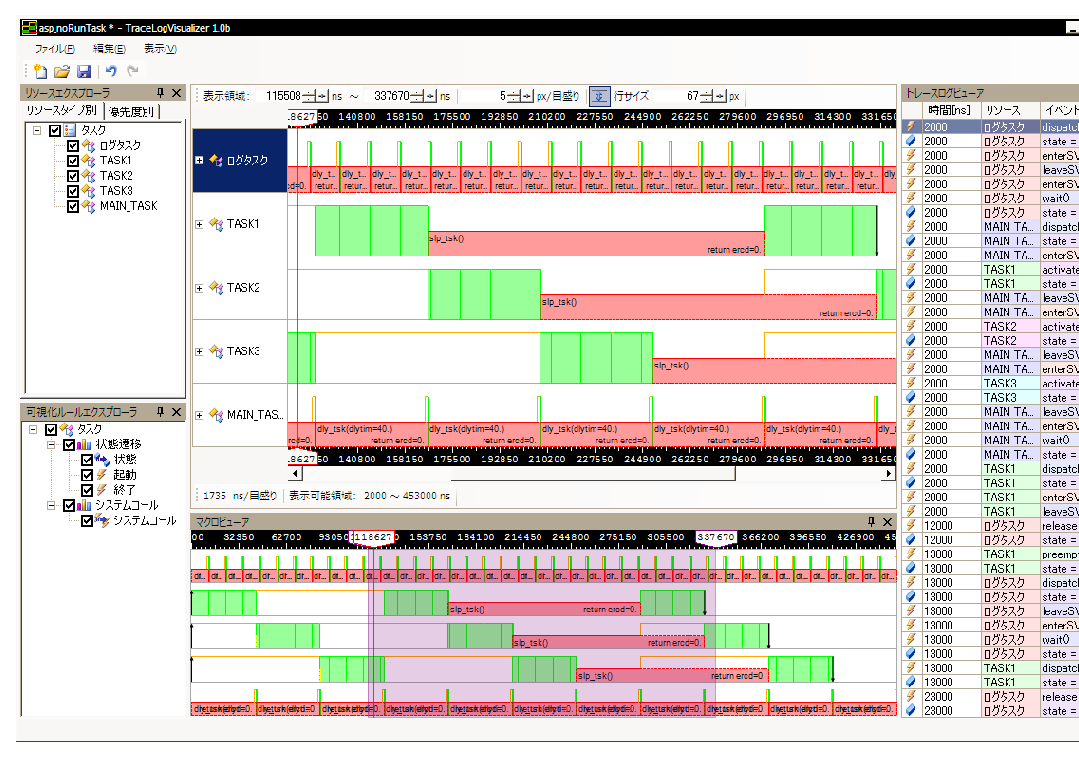
\includegraphics[width=15cm]{img/aspTLVscreenShot.eps}
\caption{TOPPERS/ASPカーネルのトレースログを可視化したTLV実行結果のスクリーンショット}
\label{fig:aspTLVscreenShot}
\end{center}
\end{figure}

図\ref{fig:aspTLVscreenShot}より,可視化表示する項目が,想定した可視化表現で描画されていることが確認できる.
たとえば,{\tt Task2}の状態が{\tt RUNNABLE},{\tt RUNNING},{\tt WAITING}と遷移し,状態が{\tt WAITING}なのは,{\tt slp\_tsk}というシステムコールを呼んで自ら待ち状態に遷移したから,ということがわかる.

\section{マルチコアプロセッサ用RTOS対応への拡張}

前小節にて,シングルコアプロセッサ用RTOSである,TOPPERS/ASPカーネルのトレースログを可視化表示できることを確認した.
本小節では,これを拡張し,マルチコアプロセッサ用RTOSである,TOPPERS/FMPカーネルのトレースログの可視化表示を試みる.

TOPPERS/FMPカーネルは,対称型(SMP)またはそれに近いマルチコアプロセッサに対応し,リアルタイム性と柔軟性を両立させたRTOSである.
タスクに対してコア間を移動させるシステムコールを実装しており,アプリケーションレベルで負荷分散を実装することが出来る.
OSが負荷分散を行わないという仕様から,各コアはシングルコアプロセッサのときと同じスケジューリング方式を用いることができるため.リアルタイム性の確保が容易になる.

TOPPERS/FMPカーネルのトレースログの形式は,ASPカーネルのものに,トレースログを記録したプロセッサIDを付与した形式になっている.
表\ref{fmpTraceLogSample}にTOPPERS/FMPカーネルのトレースログの例を示す.

\begin{File}{TOPPERS/FMPカーネルのトレースログの例}{fmpTraceLogSample}
[27526775]:[1]: enter to dly_tsk dlytim=10.
[27527154]:[2]: enter to sns_ctx.
[27527284]:[1]: task 4 becomes WAITING.
[27527390]:[2]: leave to sns_ctx state=0.
[27527518]:[1]: dispatch from task 4.
[27527622]:[2]: enter to get_pid p_prcid=1386100.
[27527714]:[1]: dispatch to task 1.
[27527814]:[2]: leave to get_pid ercd=0. prcid=2
[27528162]:[2]: enter to sns_ctx.
[27528338]:[2]: leave to sns_ctx state=0.
[27528522]:[2]: enter to get_pid p_prcid=1386144.
[27528714]:[2]: leave to get_pid ercd=0. prcid=2
\end{File}

\subsection{可視化表示する項目の追加}
\label{subsec421}

TOPPERS/FMPカーネルのトレースログを可視化するにあたり,可視化表示する項目を追加した.

FMPカーネルは,タスクが複数のコアで実行されるため,タスクがどのプロセッサに所属しているのかを可視化表示することにした.
可視化表現としては,背景を所属プロセッサ毎に色分けすることにした.
ここでは,プロセッサ1に所属している間は薄赤,プロセッサ2に所属している間は薄青とした.

\subsection{リソースヘッダファイルの修正}

所属プロセッサを可視化表現するため,リソースタイプ{\tt Task}に所属プロセッサという属性を追加する必要がある.
TOPPERS/ASPカーネル用のリソースヘッダをコピーし,表\ref{fmpResourceTypeTask}に示すように修正した.
修正内容は,ターゲットを{\tt fmp}としたこと,{\tt Attributes}の定義に{\tt prcId}を追加したことである.

\begin{File}{TOPPERS/FMPカーネル用リソースヘッダファイルの一部}{fmpResourceTypeTask}
{
  "fmp":
  {
    "Task":{
      "DisplayName" :"タスク",
      "Attributes" :{
        "prcId":{
          "VariableType"  :"Number",
          "DisplayName"  :"プロセッサID",
          "AllocationType":"Dynamic",
          "CanGrouping"  :true
        },
        ...
\end{File}

\subsection{変換ルールファイルの修正}

FMPカーネルのトレースログは表\ref{fmpTraceLogFormat}のような形式になっている.

\begin{table}[!h]
\begin{quote}
\begin{breakbox}
{\tt [}{\it time}{\tt ]:[}{\it prcId}{\tt ]: }{\it tracelog}
\end{breakbox}
\caption{TOPPERS/FMPカーネルのトレースログの形式}
\label{fmpTraceLogFormat}
\end{quote}
\end{table}

{\it prcId}がプロセッサIDであり,{\it tracelog}はASPカーネルのトレースログの時刻以降と同じである.

修正内容として,まず,検索対象となるトレースログの正規表現をプロセッサIDを考慮して修正する.
次に,実行状態のタスクを参照しているリソース記述({\tt Task(state==RUNNING)})について,プロセッサIDを条件に追加する.
これは,実行状態のタスクが最大プロセッサの数だけ存在するためである.
ASPカーネル用の変換ルールファイルを元に記述した,FMPカーネル用の変換ルールファイルの一部を表\ref{fmpConvertRule}に示す.

\begin{FileNoQuoteMini}{TOPPERS/FMPカーネル用変換ルールファイルの一部}{fmpConvertRule}
{
  "fmp":
  {
    "\[(?<time>\d+)\]:\[(?<pid>\d+)\]: dispatch to task (?<id>\d+)\." : [
      {
        "$EXIST{[${time}]Task(state==RUNNING && prcId==${pid})}"
          :"[${time}]$RES_NAME{[${time}]Task(state==RUNNING && prcId==${pid})}.state=RUNNABLE"
      },
      "[${time}]$RES_NAME{Task(id==${id})}.state=RUNNING"
    ],
    ...
\end{FileNoQuoteMini}

\subsection{可視化ルールファイルの記述}

ASPカーネル用の可視化ルールファイルは,そのまま用いることが出来る.
これは,可視化ルールファイルがトレースログの形式に依存していないからである.

\ref{subsec421}小節で述べた,所属プロセッサの可視化表示のため,FMPカーネル用に,可視化ルールファイルを追加した.
図\ref{fmpShapes}にTOPPERS/FMPカーネル用の可視化ルールファイルを示す.

\begin{FileNoQuote}{TOPPERS/FMPカーネル用の可視化ルールファイル}{fmpShapes}
{
  "fmp":{
    "VisualizeRules":{
      "taskPrcIdChange":{
        "DisplayName":"所属プロセッサ",
        "Target":"Task",
        "Shapes":{
          "prcIdChangeEvent":{
            "DisplayName":"プロセッサID",
            "When":"${TARGET}.prcId",
            "Figures":{
              "${VAL}==1":"prcIdShapes(ff0000)",
              "${VAL}==2":"prcIdShapes(0000ff)",
              "${VAL}==3":"prcIdShapes(00ff00)",
              "${VAL}==4":"prcIdShapes(ff00ff)"
            }
          }
        }
      }
    },
    "Shapes":{
      "prcIdShapes":[
        {
          "Type":"Rectangle",
          "Location":"0,0",
          "Size":"100%,100%",
          "Fill":"${ARG0}",
          "Alpha":30
        }
      ]
    }
  }
}
\end{FileNoQuote}

図\ref{fmpShapes}の内容は,まず,{\tt Shapes}で{\tt prcIdShapes}という所属プロセッサIDを示す図形を定義している.
表示領域の大きさの四角形で,引数で指定される色を塗りつぶしの色として指定している.
また,{\tt Aplha}で透明度を設定し,薄い色になるようにしている.

次に,{\tt VisualizeRules}で{\tt taskPrcIdChange}という名前で所属プロセッサを表示する可視化ルールを定義している.
イベント期間としてリソースタイプ{\tt Task}の所属プロセッサIDを表す属性{\tt prcId}の変化イベントを指定している.
その際の図形として,{\tt prcIdShapes}を指定し,変化後の所属プロセッサID({\tt prcId})の値で条件分けをして引数に与える色を変えている.
ここでは,プロセッサの数を4つまで対応できるようにした,

\subsection{実行結果}

以上のファイルの修正・追加を行い,TOPPERS/FMPカーネルのトレースログをTLVで可視化した.
図\ref{fig:fmpTLVscreenShot}にスクリーンショットを示す.

\begin{figure}[t]
\begin{center}
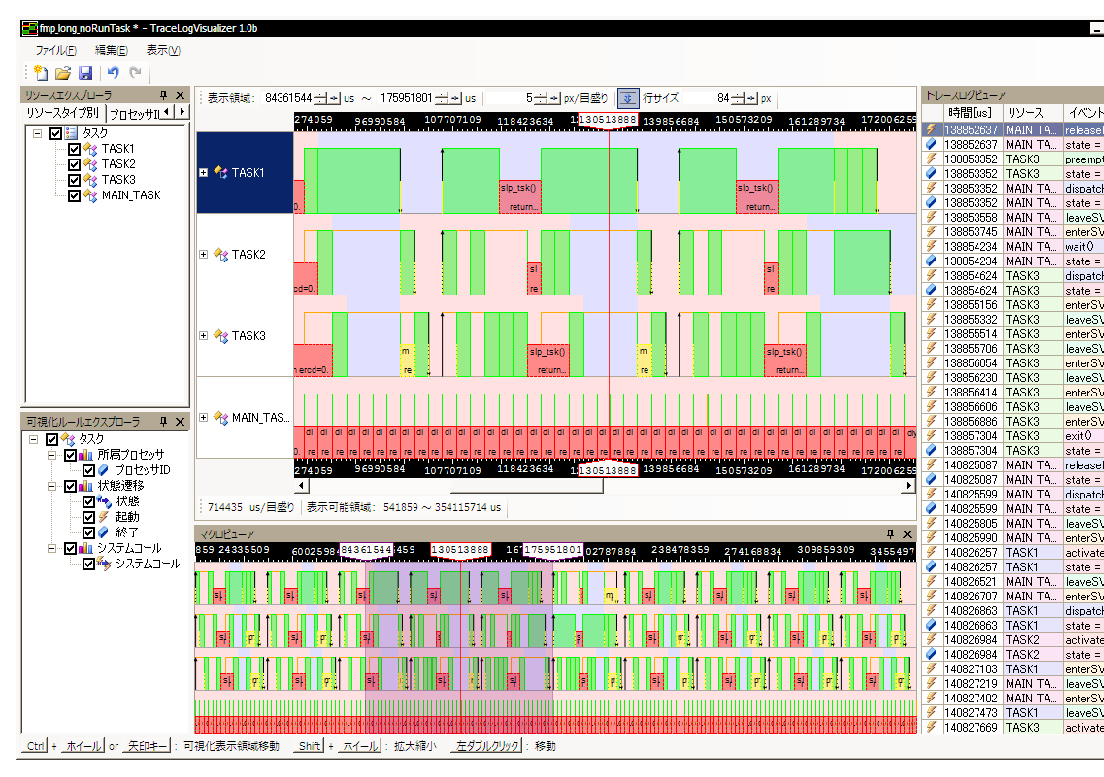
\includegraphics[width=15cm]{img/fmpTLVscreenShot.eps}
\caption{TOPPERS/FMPカーネルのトレースログを可視化したTLV実行結果のスクリーンショット}
\label{fig:fmpTLVscreenShot}
\end{center}
\end{figure}

図\ref{fig:fmpTLVscreenShot}より,各タスクの所属プロセッサにより,背景の色が分けて表示されていることがわかる.

\section{組み込みコンポーネントシステムの可視化}



\if0
\section{可視化表示項目の追加・変更}

\begin{figure}[t]
\begin{center}
\includegraphics[height=3cm]{img/runningTaskChangeVisual.eps}
\caption{実行タスクの変化の可視化表現例}
\label{fig:runningTaskChangeVisual}
\end{center}
\end{figure}

\begin{figure}[!h]
\begin{center}
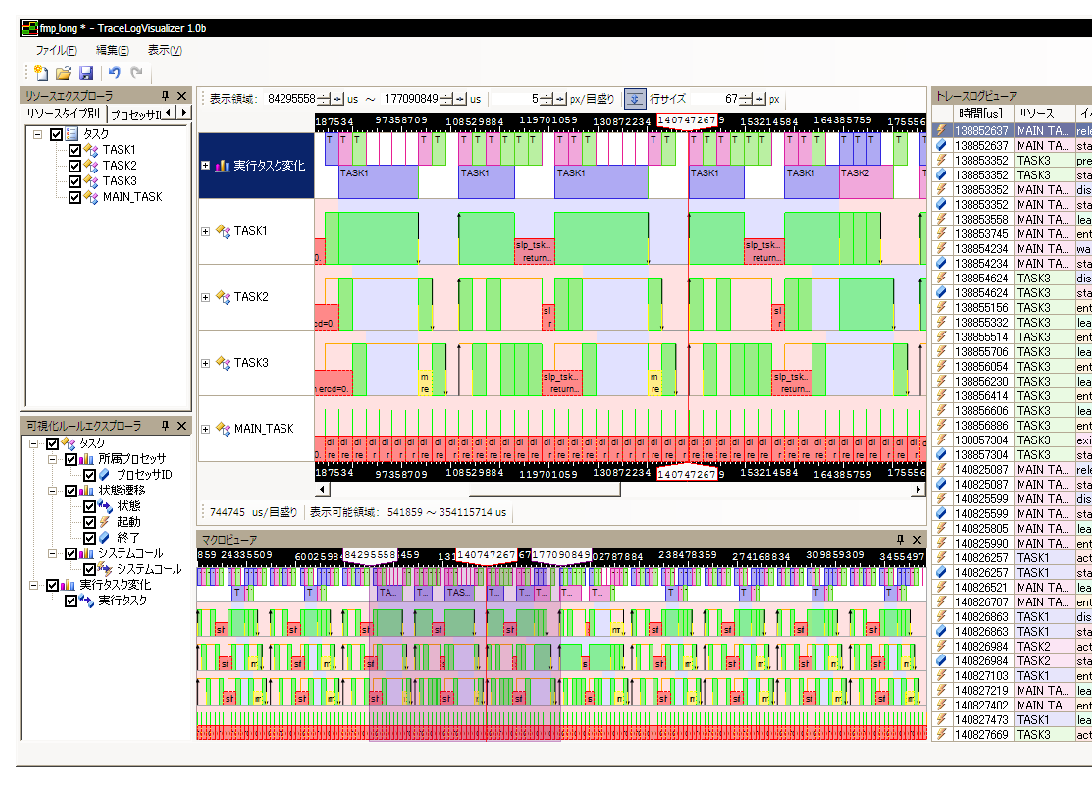
\includegraphics[width=15cm]{img/fmpRunTaskTLVscreenShot.eps}
\caption{TOPPERS/FMPカーネルのトレースログで実行タスクの変化を可視化したTLV実行結果のスクリーンショット}
\label{fig:fmppTLVscreenShot}
\end{center}
\end{figure}

実行タスクの変化の可視化表現は,四角形で,上左隅に実行タスク名を文字列を出力するとする.
また,四角形の色を実行タスク毎に変えて出力するとする.
図\ref{fig:runningTaskChangeVisual}に実行タスクの変化の可視化表現の例を示す.
実行タスクの変化を可視化している行では,時間の経過に従い,{\tt Task1},{\tt Task2},{\tt Task3}と実行状態のタスクが変化しているのがわかる.
\fi
\chapter{開発プロセス}

\section{OJL}

TLVは,OJL(On the Job Learning)の開発テーマとして開発された.
OJLとは,企業で行われているソフトウェア開発プロジェクトを教材とする実践教育であり,製品レベルの実システムの開発を通じて想像的な思考力を身につけるとともに,単なる例題にとどまらない現実の開発作業を担うことにより,納期,予算といった実社会の制約を踏まえたソフトウェア開発の実際について学ぶことを目的としている.

TLVはプロジェクトベースで開発が行われ,企業出身者2名と教員1名がプロジェクトマネージャを務め,学生3名(筆者含む)と企業出身者2名が開発実務を行った.
進捗の報告は,週に1度のミーティングと週報の提出により行った.

\subsection{フェーズ分割}

単年度でTLVを開発するにあたり,全体を3フェーズに分割した.
各々のフェーズの内容は次の通りである.

\subsubsection{フェーズ1}

\begin{description}
\item[期間] \mbox{} \\
2008年5月~同年8月(約3ヶ月)

\item[目的・目標] \mbox{} \\
プロトタイプの実装を行い,そのプロセスと成果物から,GUIの評価や要求の再抽出,アプリケーションドメイン分析を通じた設計方法の探索を行う.

\item[実装内容] \mbox{} \\
機能を限定して実装を行う.

トレースログの対象をTOPPERS/ASPカーネルに絞り,可視化表示項目もタスクの状態遷移のみとする.

標準形式トレースログへの変換や,可視化ルールの適用による可視化表示は行わない.

\item[実施結果] \mbox{} \\
実装成果物の総行数は約9000行(有効行数5000行)であった.

開発関係者4名とRTOS開発者および利用者の7名に成果物を利用してもらい意見を収集した.
その結果,ユーザインタフェース,追加の機能要求,可視化表現項目について意見が得られた.

実装中心の開発プロセスになってしまい,チーム開発がうまく機能しなかった.

\end{description}

\subsubsection{フェーズ2}

\begin{description}
\item[期間] \mbox{} \\
2008年9月~2009年1月(約5ヶ月)

\item[目的・目標] \mbox{} \\
標準形式トレースログの策定,可視化ルールの策定.
標準形式トレースログへの変換,可視化ルールファイルによる可視化表示の外部プラグイン化の実装.
ユースケース駆動アジャイル開発の導入.

\item[実装内容] \mbox{} \\
主要機能である,標準形式トレースログへの変換,可視化ルールファイルによる可視化表示の外部プラグイン化を実装する.
また,フェーズ1にて再定義された機能要求を可能な限り実装する.

\item[実施結果] \mbox{} \\
実装成果物の総行数は約18500行(有効行数10300行)であった.

標準形式トレースログ,可視化ルールファイル,またリソースファイル,リソースヘッダファイルの形式を本論文で述べたとおり定義した.

また,本論文で示したとおり,標準形式トレースログへの変換と可視化ルールファイルによる可視化表現項目の追加を実現できた.

ユースケース駆動アジャイル開発により,ユースケース毎にイテレーションを繰り返し実施し開発を行った.
結果,36個中27個のユースケースについて実装が完了した.

\end{description}

\subsubsection{フェーズ3}

\begin{description}
\item[期間] \mbox{} \\
2008年2月~2009年3月(約1ヶ月)

\item[目的・目標] \mbox{} \\
TLVで読み込めるトレースログ形式を増やす.
可視化表現項目を増やす.

\item[実装内容] \mbox{} \\
フェーズ2の成果を元に,変換ルールファイルを追加・変更し対応するトレースログの形式を増やす.また,可視化ルールファイルを追加・変更し可視化表現項目の充実を図る.

\item[実施結果] \mbox{} \\
未実施である.

\end{description}


\section{ユースケース駆動アジャイルソフトウェア開発}
\label{usecaseAgile}

フェーズ2において,TLVの開発は,ユースケース駆動アジャイルソフトウェア開発という手法を用いて行われた.

アジャイルソフトウェア開発では,反復(イテレーション)と呼ばれる短い期間を単位に反復して開発を行い,計画ではなく状況において適応的に対応することを重視してソフトウェア開発を行う.
1つのイテレーション内では1つの機能に対して設計,実装,テスト,文書化といった工程を完結して行う.
TLVの開発ではユースケースを機能の単位にイテレーションを反復して実施した.
図\ref{fig:agile}にユースケース駆動アジャイルソフトウェア開発の例を示す.

\begin{figure}[t]
\begin{center}
\includegraphics[scale=0.75]{img/agile.eps}
\caption{ユースケース駆動アジャイルソフトウェア開発}
\label{fig:agile}
\end{center}
\end{figure}

はじめに外部設計としてユースケース図,ユースケース内のクラス図,シーケンス図を作成する.
次に,クラス単位で内部設計,単体テスト,実装を行う.
内部設計では,クラス図で定義したクラスに関してインタフェースのみを記述したスケルトンを作成し,コメントとして内部設計を記述する.
単体テストは,メソッド単位のユニットテストとし,統合開発環境に付属するユニットテストフレームワークを用いて実装,実施する.
単体テストの実装はテストケースの記述であり,ユニットテストフレームワークが出力するテストコードのスケルトンに必要な情報を記述することで行う.
単体テストの実装が終わったらクラスの実装を行う.
クラスの実装は,単体テストを実施しながら,テスト項目のをすべてを成功するかどうか試しながら行う.
1つのクラスの実装が終わればユースケース内の次のクラスの内部設計に移る.

このようにしてユースケース内のクラスをすべて実装したら,ユースケース内のクラスを結合してユースケースとして駆動する形に実装する.
この際も,テストケースの実装を先に行ってから実装を開始する.
結合テストのテスト項目のをすべてを成功したら,1つのイテレーションの完了であり,次のユースケースの外部設計を開始する.

本節では,TLVの開発において,ユースケース駆動アジャイルソフトウェア開発の各工程で実践した内容について詳述する.

\subsection{プロジェクト管理}

フェーズ2のはじめの作業として,フェーズ1で行った評価の結果と,フェーズ2の実施概要について,プロジェクト計画書として文書化した.

次に,フェーズ2で実装するTLVの機能を,要求仕様書として文書化した.
また,機能をユースケースを単位に定義し,ユースケース図を作成した.
図\ref{fig:usecase}にTLVのユースケース図を示す.

\begin{figure}[t]
\begin{center}
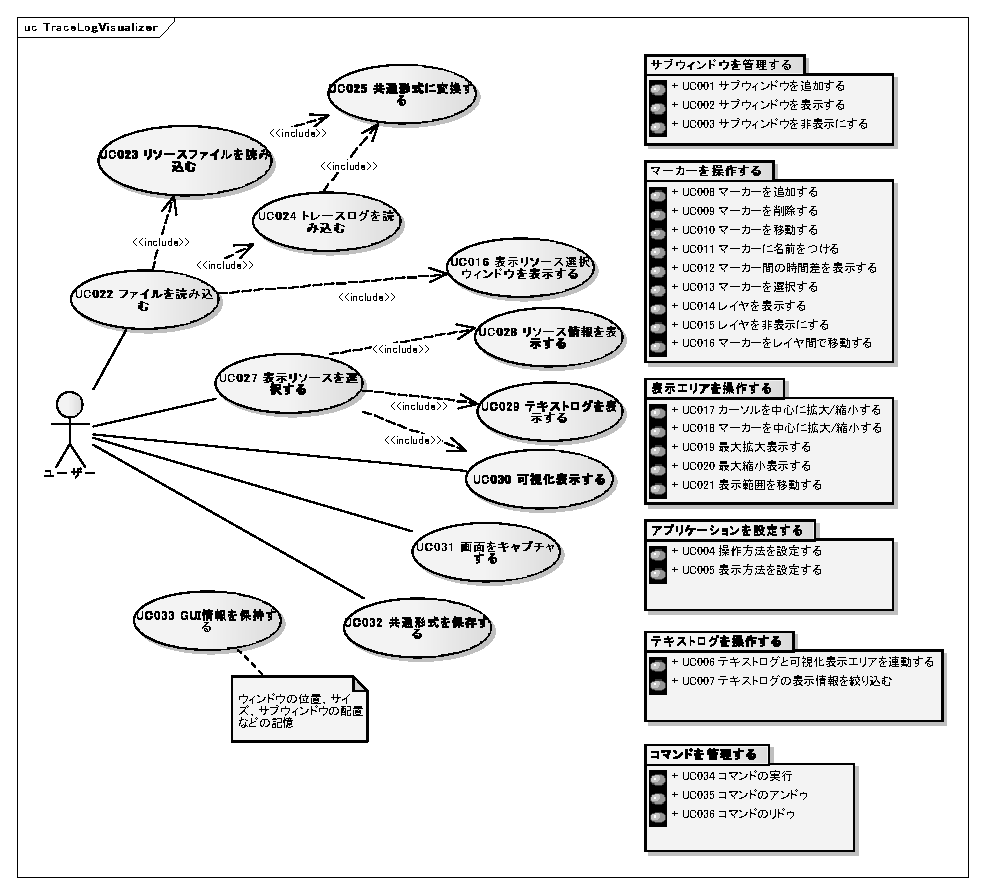
\includegraphics[scale=0.75]{img/usecase.eps}
\caption{TLVのユースケース図}
\label{fig:usecase}
\end{center}
\end{figure}

TLVの機能をユースケースを単位に定義した結果,全ユースケース数は36個であった.
これらのユースケースを工程毎に分けた進捗表を作成し,これを用いて進捗管理を行い,複数のメンバーで工程の分担,作業項目の同期を行った.

\subsection{設計}

図\ref{fig:agile}に示すとおり,外部設計としては,ユースケース内のクラスについて,クラス図を,クラス間の連携の流れをシーケンス図として作成することで行う.
図\ref{fig:class}に作成したクラス図の例を示す.
また,図\ref{fig:sequence}に作成したシーケンス図の例を示す.

\begin{figure}[t]
\begin{center}
\includegraphics[width=13cm]{img/class.eps}
\caption{TLVの外部設計で作成したクラス図の例}
\label{fig:class}
\end{center}
\end{figure}

\begin{figure}[t]
\begin{center}
\includegraphics[width=13cm]{img/sequence.eps}
\caption{TLVの外部設計で作成したシーケンス図の例}
\label{fig:sequence}
\end{center}
\end{figure}

内部設計は文書化せずに,ソースコードのコメントを記述することで行った.
外部設計で作成したクラス図を元に,インタフェースのみを記述したクラスを記述し,メソッドのコメントとして,引数,返値の説明,どのような内部実装を行うべきかの説明を記述する.

\subsection{テスト}

TLVのテストは,統合開発環境に付属するユニットテストフレームワークを用いて実装,実施した.
ユニットテストフレームワークは,クラスのメソッドの定義を元に,テストケースのスケルトンを自動生成する仕組みを搭載しており,テスト工程作業の大幅な省力化を図ることができる.
スケルトンは,引数の組み合わせと期待値を開発者が入力するように生成されており,これらを入力する作業が実質的なテストケースの実装作業となる.

ユニットテストの単位はメソッドだが,単純なアクセサメソッドはテストの対象外とした.
その結果,491メソッドがユニットテストの対象となった.

\subsection{実装}

TLVの実装言語は,C$\sharp$ 3.0である.
統合開発環境として Microsoft Visual Studio 2008 Professional Edition を用いた.
TLVの実行には .NET Framework 3.5 が必要である.

実装はクラス単位で行い,ユニットテストが全部成功することを目標に行う.
その際,テストの実施とクラスの実装は反復して行う.
テスト結果は記録されるため,文書化する必要がなく,素早くデバッグを行うことができる.

TLVのソースコードメトリクスを表\ref{sourceMetrics}に示す.

\begin{table}[htb]
\begin{center}
\begin{tabular}{l|l}
\hline
総行数              & 18497 \\
ファイル平均行数    & 94.38 \\
有効な行数          & 10332 \\
コメント行数        & 1432 \\
空行                & 2224 \\
その他の行数(中括弧など) & 4509 \\
ファイル数          & 196 \\
クラス数            & 186 \\
構造体数            & 0 \\
インタフェース数    & 22 \\
列挙体              & 15 \\
デリゲート          & 2 \\
\hline
\end{tabular}
\caption{TLVのソースコードメトリクス}
\label{sourceMetrics}
\end{center}
\end{table}


\chapter{開発スタイル}

\section{OJL}

\subsection{フェーズ分割}

\section{ユースケース駆動アジャイル開発}

\subsection{プロジェクト管理}

\subsection{設計}

\subsection{テスト}

\section{開発成果物}

\chapter*{謝辞}
\addcontentsline{toc}{chapter}{謝辞}

TLVを開発するにあたり,ご指導を賜りました名古屋大学大学院情報科学研究科情報システム学専攻組み込みリアルタイムシステム研究室の高田広章教授,同研究室の冨山宏之准教授に深く感謝致します.
また,開発プロジェクトマネージャとして日頃より多くのご助言を頂きました同研究室の本田晋也助教,同研究科付属組込みリアルタイム研究センターの長尾卓哉研究員に深く感謝致します.

TLVのテストに関して,テスト仕様の作成から実施までご尽力頂きました名古屋大学大学院情報科学研究科情報システム学専攻阿草・結縁研究室の水野洋樹氏,同専攻宮尾・八槇研究室の柳澤大祐氏に深く感謝いたします.

 

 

 

 

 

杉本さん記述すること
\begin{thebibliography}{99}
%\addcontentsline{toc}{chapter}{\bibname}
\bibitem{PARTNER-JET}
JTAG ICE PARTNER-Jet,http://www.kmckk.co.jp/jet/,最終アクセス2009年1月14日

\bibitem{watchpoint}
WatchPointデバッガ,https://www.sophia-systems.co.jp/ice/products/watchpoint,最終アクセス2009年1月14日

\bibitem{QNXMomentics}
QNX Momentics Tool Suite,http://www.qnx.co.jp/products/tools/,最終アクセス2009年1月14日

\bibitem{eBinder}
eBinder,http://www.esol.co.jp/embedded/ebinder.html,最終アクセス2009年1月14日

\bibitem{LKST}
LKST(Linux Kernel State Tracer) - A tool that records
traces of kernel state transition as events,http://oss.hitachi.co.jp/sdl/english/lkst.html,最終アクセス2009年1月14日

\bibitem{SystemTap}
Prasad, V., Cohen, W., Eigler, F. C., Hunt, M., Keniston, J. and Chen, B.: Locating system problems using dynamic instrumentation. Proc. of the Linux Symposium, Vol.2, pp.49–64, 2005.

\bibitem{LTTng}
Mathieu Desnoyers and Michel Dagenais.: The lttng tracer : A low impact performance and behavior monitor for gnu/linux. In OLS (Ottawa Linux Symposium) 2006, pp.209–224, 2006.

\bibitem{Dtrace}
R. McDougall, J. Mauro, and B. Gregg.: Solaris(TM) Performance and Tools: DTrace and MDB Techniques for Solaris 10 and OpenSolaris. Pearson Professional, 2006.

\bibitem{LTTV}
Mathieu Desnoyers and Michel Dagenais.: OS Tracing for Hardware, Driver and Binary Reverse Engineering in Linux. CodeBreakers Journal Article, vol.4, no.1, 2007.

\bibitem{Chime}
OpenSolaris Project: Chime Visualization Tool for DTrace,http://opensolaris.org/os/project/dtrace-chime/,最終アクセス2009年1月14日

\bibitem{RFC3164}
RFC3164 The BSD syslog Protocol, http://www.ietf.org/rfc/rfc3164.txt,最終アクセス2009年1月14日

\bibitem{Json}
RFC4627 The application/json Media Type for JavaScript Object Notation (JSON),http://tools.ietf.org/html/rfc4627,最終アクセス2009年1月14日

\bibitem{TOPPERS}
TOPPERS Project,http://www.toppers.jp/,最終アクセス2009年1月14日

\bibitem{TECS}
Takuya Azumi and Masanari Yamamoto and Yasuo Kominami and Nobuhisa Takagi and Hiroshi Oyama and Hiroaki Takada.:A New Specification of Software Components for Embedded Systems. Proceedings of the 10th IEEE International Symposium on Object and Component-Oriented Real-Time Distributed Computing (ISORC 2007), pp.45-50, 2007

\end{thebibliography}

\input{src/appendix.tex}
\clearpage
%%%%%%%%%%%%%%%%%%%%%%%%%%%%%%%%%%%%%%%%%%%%%%%%%%%%%%%%%%%%%%%%%%%%%%%%%%
% 背表紙
%-------------------------------------------------------------------------
\thispagestyle{empty}
\oddsidemargin -4in
\evensidemargin -4in
\topmargin -.5in
{
\tate
\Large\sffamily\gtfamily
\begin{minipage}{9.5in}
\begin{minipage}{6.0in}
OJLによるトレースログ可視化ツールの開発
\end{minipage}
\hfill\hfill\hfill\hfill
350702101
\hfill
後藤 隼弐
\end{minipage}
}
\end{document}
